\appendix

\section{Project directive and templates}
	
	\subsection{Contact information}
		\subsubsection{Customer}
			\begin{itemize}
				\item {\bf Nils Valland} \newline
						Telephone: 73 59 23 01 \newline
						Mobile: 92 41 20 37 \newline
						Fax: 73 59 22 40 \newline
						E-mail: nils.valland@artsdatabanken.no
				\item {\bf Askild Olsen} \newline
						Telephone: 73 59 21 93 \newline
						Mobile: 91 78 34 89 \newline
						Fax: 73 59 22 40 \newline
						E-mail: askild.olsen@artsdatabanken.no
			\end{itemize}
			
		\subsubsection{Supervisor}
			\begin{itemize}
				\item {\bf Muhammad Asif} \newline
						Telephone: 73 59 36 71 \newline
						E-mail: muhamma@idi.ntnu.no
			\end{itemize}

		\subsubsection{Team members}
				\begin{itemize}
					\item {\bf Anders Sbstad Rye} \newline
							E-mail: anders.rye@gmail.com
					\item {\bf Andreas Berg Skomedal} \newline
							E-mail: aokaado@gmail.com
					\item {\bf Dag-Inge Aas} \newline
							E-mail: daginge@gmail.com
					\item {\bf Muhsin Gnaydin} \newline
							E-mail: gunaydim@gmail.com
					\item {\bf Nikola Djoric} \newline
							E-mail: nikola.djoric@gmail.com
					\item {\bf Stian Liknes} \newline
							E-mail: stianlik@gmail.com
					\item {\bf Yonathan Redda} \newline
							E-mail: chenecx@gmail.com
				\end{itemize}
				
	\subsection{Meeting agendas}
		\begin{figure}[htb]
			\centering
			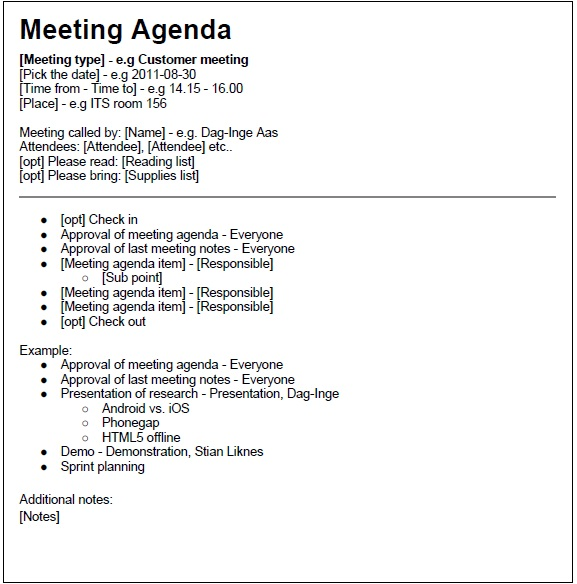
\includegraphics[width=0.8\textwidth]{appendix/meeting_agenda.jpg}
			\caption{Meeting agenda}
			\label{fig:meeting-agenda}
		\end{figure}
	
	\newpage
	\subsection{Meeting minutes}
		\begin{figure}[htb]
			\centering
			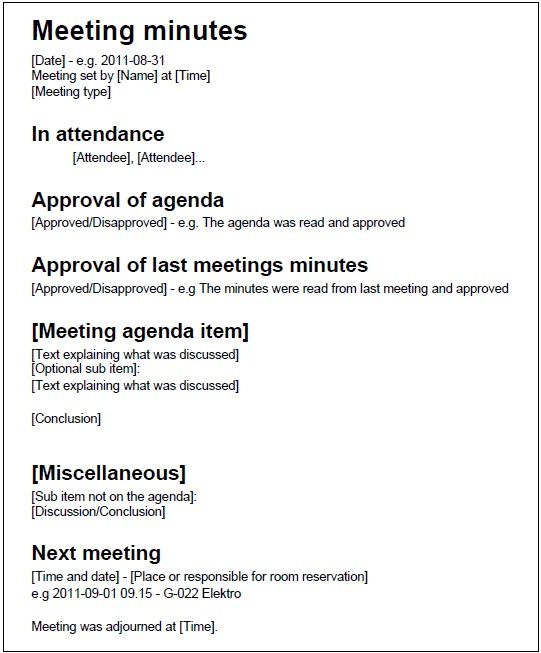
\includegraphics[width=0.8\textwidth]{appendix/meeting_minutes.jpg}
			\caption{Meeting minutes}
			\label{fig:meeting-minutes}
		\end{figure}
	
	\newpage
	\subsection{Weekly status report}
		\begin{figure}[htb]
			\centering
			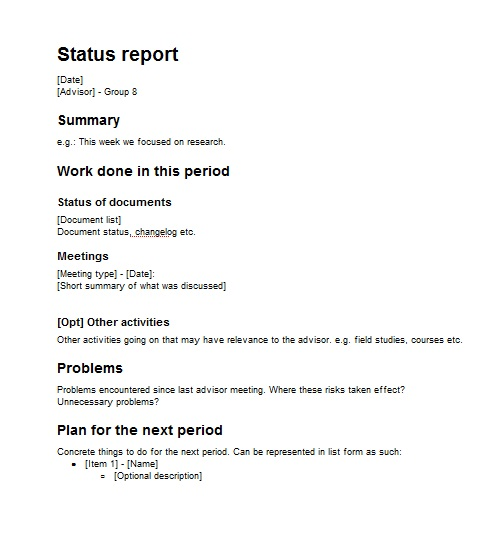
\includegraphics[width=0.8\textwidth]{appendix/weekly_status_report.jpg}
			\caption{Weekly status report}
			\label{fig:weekly-status-report}
		\end{figure}

\newpage
\section{User guide TODO}
This portion of the document details installation guides for the user, in addition to a how-to for the application. This should provide the user with adequate information about how to install and use the application.
\subsection{Installation guide}
The application can be downloaded from the Android Market, with the name "Artsdatabanken". It can also be installed directly from an executable installation package, an apk, by going to the following url: \url{http://stuff.daginge.com/artsdatabanken.apk}.

However, if the user wishes to install the latest build, see Developers guide.

\subsection{How-to}
\subsubsection{Creating an observation}
The user creates an observation by following the "Create and observation" link from the front page of the application. From here, the user selects which species group to observe. This will lead the user to an observation table, where the user can input species name, which is auto-completed, and the number of individuals found. Both common names and scientific names are applicable. From here, the user can choose to add more information about the species observation by selecting "Add more information".

\subsubsection{Storing an observation TODO}
This will come

\subsubsection{Editing a stored observation TODO}
More to come

\subsubsection{Exporting an observation TODO}
Come here you little

\section{Developers guide TODO}
This section will in details help maintaining developers understand and use the code we have produced during the course of this project. It will also include comments about the ideas we have for the further development of this app.

\subsection{Further work}
A small text about the further potential of this app, and what it is now.
\subsubsection{Use of API}
Use of artsdatabankens api in our application.

\subsubsection{Code repository}
The code and documentation from this project can be found in its entirety at the follwing url: \url{https://github.com/cdproject8/Artsdatabanken}. Included here is a complete revision history for our entire project, all of our documentation excluding meeting minutes and agendas, in addition to the app itself. The application is ready to compile from this source.

For further work, we recommend you fork this project. The project is licensed under Creative Commons Attribution-ShareAlike 3.0 Unported, and all further work should also be licensed under the same or similar licenses. 

\subsubsection{Maintenance}
A short text about maintenance, and the challenges ahead.

\subsubsection{Not yet implemented and ideas}
Ideas for further development of the app from the project group and customer.

